\section{The research question}\label{sec:question}

\subsection{Background: two pulls on the same nights}

On an ordinary weekday night in February 2024, about 2.1 million residents of mainland Spain slept in a zone other than their own. On the night of 14 to 15 August, 8.5 million did. Groups of at least 10 residents of Madrid slept in 2,203 of the other 2,434 zones that night, against 1,124 in February. Many of the places that received them are villages that lost most of their people in the twentieth century. In this report I try to find out where all these people go, and whether the old migration from the villages still has something to do with it.

Between 1950 and 1975 Spain went through what historians call its \emph{rural exodus}: a mass move from the villages of the interior to the cities. About two million people left the countryside in the 1960s alone \citep[p.~225]{clar2023rural}. Municipalities under 2,000 inhabitants were home to more than 11 million people in the 1950s and to about 7 million in 2017 \citep[p.~5]{pinilla2017rural}. The emigrants came mainly from the rural south and interior and settled in Madrid, Catalonia and the Basque Country \citep{bover1999migrations}. Many kept a house in the village, and in Spain people still talk of \es{volver al pueblo}, going back to the village, in August. About 15.5\,\% of Spanish households had a second home in 2021 \citep{ine2023ecepov}, and in the third quarter of 2024, 28.3\,\% of the trips made by residents were visits to relatives or friends \citep{ine2024etr3t}.

But August is also beach season, so my first worry was that the beach would simply win. Figure~\ref{fig:calendar} shows that it does not. Outside August, on 149 of the 150 nights of 2024 with data (dating each night by its evening), more of the people who sleep at least 100\,km from their home zone (in a straight line between zone centres) do so in inland towns and villages than in coastal zones, those that touch the sea. In August the coast is slightly ahead on almost every night, but the two stay close: on the night of 14 to 15 August, 2.2 million people slept far from home on the coast and 2.1 million in inland towns and villages.

\begin{figure}[t]
\centering
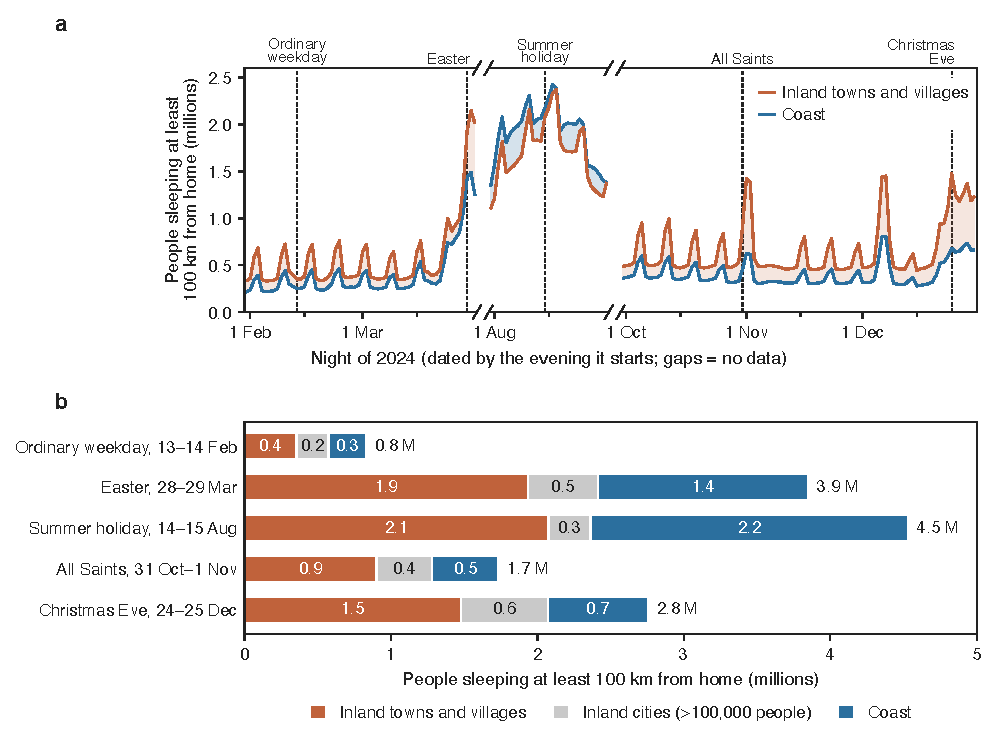
\includegraphics[width=\linewidth]{fig1_option2_calendar.pdf}
\caption{\textbf{Where people sleep when they are far from home.} \textbf{a}, People sleeping at least 100\,km from their home zone on each night of 2024 with data, in inland towns and villages (terracotta) and in coastal zones (blue); the shading marks which received more. Dashed lines mark the five nights studied; gaps are months without data. \textbf{b}, The five nights, in millions of people, with inland cities of more than 100,000 people in grey. Easter is the night ending on Good Friday. Data: overnight-stay estimates of the Spanish Ministry of Transport (MITMA) for 2,435 mainland zones.}
\label{fig:calendar}
\end{figure}

So both pulls are large, and just counting people cannot answer the question: a person sleeping in an inland village in August may be visiting the family home or hiking in the mountains. The generation that left in the 1960s is now old, and their children and grandchildren were born in the cities. The ties to the village may have faded, or moved to an apartment by the sea. Holidays may also just make the network denser everywhere, with no preference for any destination. What I need to look at is not how many people travel but \emph{who goes where}: whether the residents of a city sleep, on holiday, in the provinces and villages its population came from.

\subsection{The networks studied}

The data are the overnight-stay estimates of the Spanish Ministry of Transport \citep{mitms2024methodology}. For each night, they estimate from mobile-phone records how many residents of each zone slept in each other zone, scaled up to the whole population. A zone is a municipality (the local administrative unit, from a village to a city), or a group of small neighbouring municipalities: the 2,435 zones of mainland Spain cover 7,975 municipalities and 43.9 million residents. Municipalities are grouped into 47 mainland provinces, which are the unit of birthplace below. I build one network per night:
\begin{itemize}
\item \textbf{Nodes:} the 2,435 zones.
\item \textbf{Links:} a directed link from zone $i$ to zone $j$ when at least 10 residents of $i$ sleep in $j$ that night. The number of people is kept as the link weight.
\end{itemize}
I added the threshold because many links carry only one or two estimated people, which is mostly noise. It keeps between 69\,\% and 83\,\% of the people who sleep away from home, and leaves networks with 0.9--3.4\,\% of all possible undirected links (Section~\ref{sec:method}).

I use single nights rather than averages over a holiday period, because an average mixes the people who leave with those who come back. The three main networks are an ordinary weekday (the night of 13 to 14 February), the summer holiday (14 to 15 August, the eve of a national holiday at the peak of the summer break) and All Saints (31 October to 1 November, a national holiday when families traditionally visit their relatives' graves), when the coast pulls less. Christmas Eve and Easter appear where they help. Each main night is checked against comparable nights of the same period, which I call its \emph{sister nights} (Section~\ref{sec:method}), and against the same dates in 2022 and 2023.

A second kind of network records where residents were born. For each municipality with more than 10,000 residents, the 2024 census records how many of its residents were born in each province, when they arrived in their current province, and how large their municipality of birth was \citep{ine2025censo}. This gives a \emph{roots network}: a link from a municipality to a province, weighted by the number of its residents born there. To compare the two, I add up the overnight stays from each of these municipalities that is a zone of its own to each other province, so that both networks link the same cities to the same provinces.

\clearpage
\subsection{The research question and tasks}

The question is:

\begin{quote}
\emph{On holiday, do Spaniards go back to the villages their families left?}
\end{quote}

Put in network terms: compared with an ordinary night, does the overnight-stay network of the holidays lean towards the provinces where the residents of each city were born, and towards the \emph{emptied villages}, the zones that lost the largest share of their 1900--1960 peak population, beyond what distance, income and the coast explain? I split it into four tasks.

\begin{enumerate}[label=\textbf{T\arabic*.}]
\item \textbf{Describe the networks.} Measure their basic properties (degree distribution, path length, clustering, mixing, rich club) and compare them with random networks that keep the same number of links per zone.
\item \textbf{Compare holiday and ordinary nights.} Find out whether the holiday network changes shape, and whether the change is more than what its new degrees force, using the rewiring methods of \citet{zhou2007structural}.
\item \textbf{Compare the overnight network with the roots network.} Test whether a city sends more of its residents to the provinces where more of them were born, comparing cities of the same province against the same destination province, with the distance from each city modelled, and whether that pull grows on holiday and for which generation.
\item \textbf{Look at the villages.} Test whether the most emptied zones switch from sending people away to receiving them.
\end{enumerate}

\subsection{Why this question is worth studying}

Apart from being something I was curious about, the question matters outside this course too. The villages emptied by the exodus have few registered residents, and much of what is known about them comes from that register. People who sleep in a family home or a second home may also escape hotel statistics. \citet{garciagonzalez2024retorno} measured this \emph{return tourism} with phone data in one region, Castilla-La Mancha. A national picture of who comes back, from where and when, describes a part of rural Spain that the usual statistics miss.

It also fits a network course well, for three reasons. First, it is about links, not places: the same number of visitors to a village can come from its emigrants or from strangers, and only where visitors live, set against where that place's residents were born, can tell them apart. Second, it compares networks on common units, holiday against ordinary and overnight against roots, which is the comparison network methods are built for. Third, the holiday network is much denser than the ordinary one, so any of its properties could change just because of its size. Random networks that keep each zone's number of links separate what the new degrees force from what they do not.

The closest earlier work is a study of the Chinese Spring Festival, which compared travel between 31 provinces with the census network of where migrants come from \citep{li2016spring}. With 31 provinces that network is almost complete, so it says little about structure, and the comparison has no control for distance. Studies of Spanish phone data have described seasonal changes in population \citep{garzon2026heritage} and return tourism in one region \citep{garciagonzalez2024retorno}, but without birthplaces or networks. I could not find a study that measures the structure of the network of where Spaniards sleep on holiday, or compares its flows with where the cities' residents were born, so that is what I try to do here. Section~\ref{sec:literature} discusses these and other works in detail.
